\chapter{System Overview} \label{chap:system_overview}

\begin{figure}
\center
	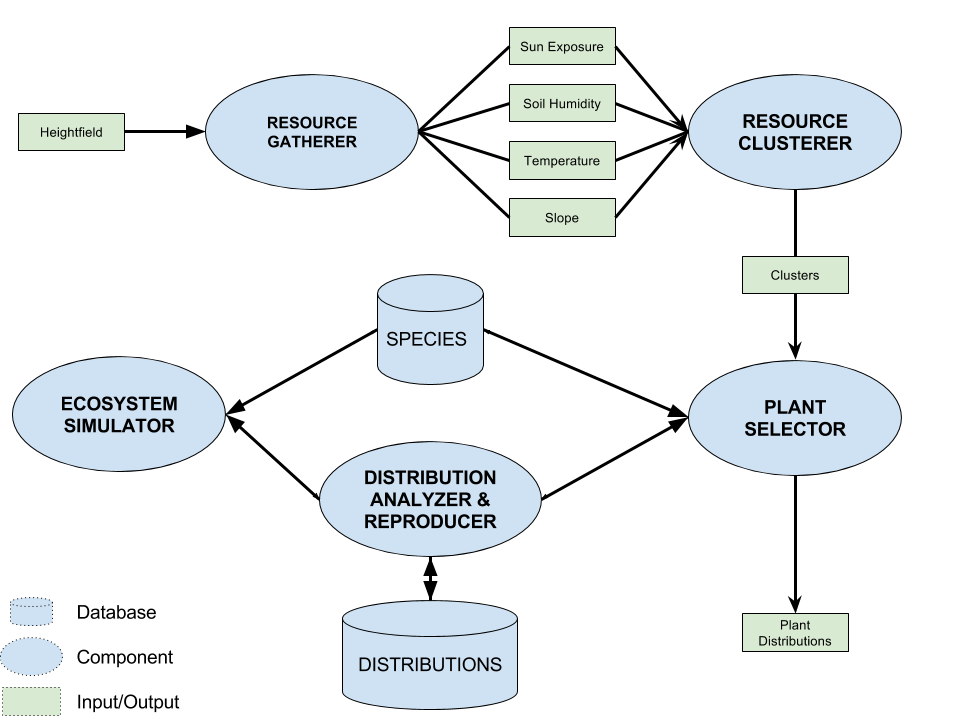
\includegraphics[width=\textwidth]{system_overview.png}
	\caption{\textit{System overview}}	
	\label{fig:system_overview}
\end{figure}

Multiple components serving specific purposes constitute the building blocks of the overall system, notably: \textit{resource gathering}, \textit{resource clustering}, \textit{plant selection}, \textit{ecosystem simulation} and \textit{distribution analysis and reproduction}. The purpose of this chapter is to give an overview of the system, each component and how they fit together (as illustrated in figure \ref{fig:system_overview}). To do so, an overview of each component is provided separately along with it's purpose, required inputs and outputs.\\
To conclude, the \textit{limitations} of the system will be discussed and \textit{comparisons and differences} drawn with previous work in the field.

\section{Resource Gatherer} \label{sec:resource_gatherer}

Vegetation requires resources to grow and the distribution of these resources identifies a given species and associated it with a given climate and, subsequently, location on earth. Determining resource data is essential, therefore, to generating realistic virtual worlds as it is vital to determining vegetation distribution patterns. The purpose of the resource gatherer is to determine, for each terrain vertex: \textit{sun exposure}, \textit{soil humidity}, \textit{temperature} and \textit{slope}. Figure \ref{fig:system_overview_resource_gatherer} illustrates the output of the resource gatherer along with the user inputs required.\\
The latitude and orientation of the terrain must be specified by the user in order to determine the sun position throughout the year. The \textit{sunlight exposure} calculation then determines, given this information and the terrain relief, the average daily illumination (in hours) received by each terrain vertex for each month of the year. To calculate the average illumination for a given month, the trajectory of the sun is calculated for the fifteenth day. \\
In order to calculate the \textit{soil humidity} for each month, the soil infiltration rate, monthly rainfall quantity and monthly rainfall intensity must be configured.\\
To determine the \textit{temperature} of each terrain vertex, the user must specify the temperature at zero metres in June and December along with the associated lapse rate. These temperatures are then considered the annual minimum and maximum and are used to deduce the temperature for any month through linear interpolation. The lapse rate represents the decrease in temperature with altitude and is used to determine the temperature for any terrain vertex given its altitude. \\
The \textit{slope} is determined automatically from the input terrain.\\

\begin{figure}
\center
	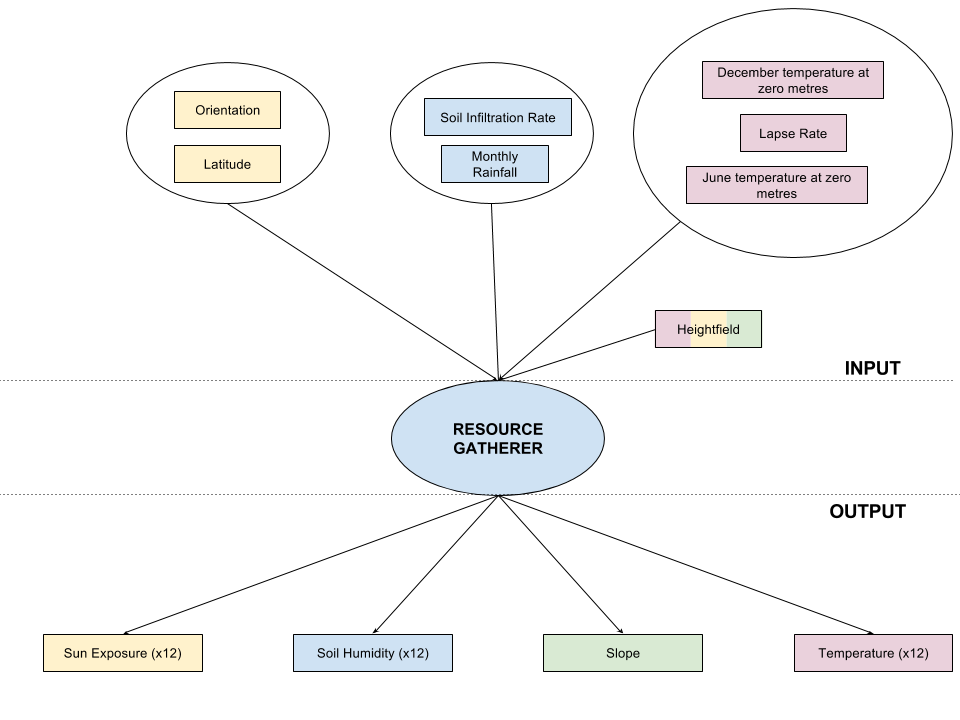
\includegraphics[width=\textwidth]{system_overview_resource_gatherer.png}
	\caption{ \textit{Resource gatherer overview with colour coding to correlate input with corresponding output.}}	
	\label{fig:system_overview_resource_gatherer}
\end{figure}

\section{Resource Clusterer}

Determining a suitable plant distribution for each individual terrain vertex is infeasible due to the associated computation cost. To reduce the amount of plant distributions to calculate, K-means clustering is performed on the terrain to group together points with similar resource properties. The mean value of each cluster is then used to determine suitable vegetation and its distribution. Figure \ref{fig:system_overview_resoure_clusterer} illustrates the input requirements and output of this component.\\
The \textit{cluster count} which must be specified as input dictates how many clusters the algorithm produces. In essence, it controls the sensitivity of the clustering algorithm.\\
The per-vertex resource data represents all the resource information discussed in section \ref{sec:resource_gatherer}.\\
Given all this information, the clustering algorithm gathers points which are most similar in terms of resources into a set of \textit{k} clusters. \\

\begin{figure}
\center
	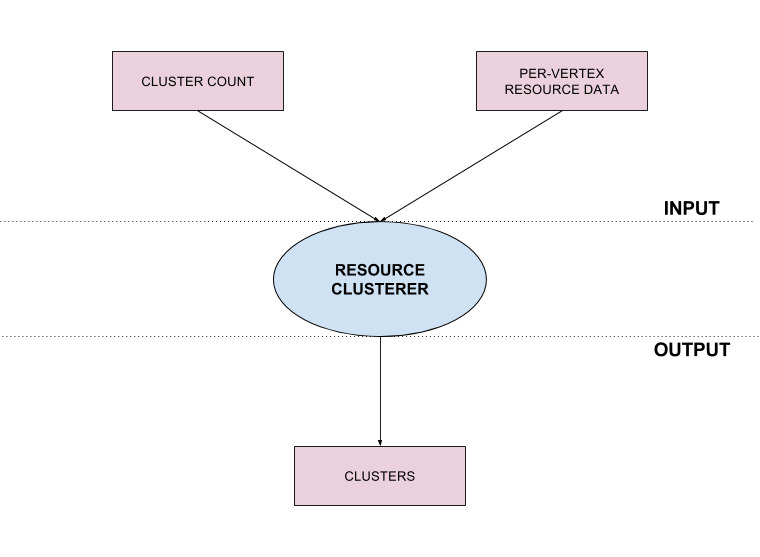
\includegraphics[width=\textwidth]{system_overview_resource_clusterer.png}
	\caption{ \textit{Resource clusterer overview with required input and generated output.}}	
	\label{fig:system_overview_resoure_clusterer}
\end{figure}

\section{Plant Selector}

Given the mean value of the individual clusters, the plant selector determines the plants which are able to survive in each terrain cluster and calculates for each of them a suitability score. This score depicts how suited a species is to each individual cluster and is displayed to the user for informational purposes in order to facilitate the species selection procedure. Figure \ref{fig:system_overview_plant_selector} shows the input requirements and outputs of this component.

\begin{figure}
\center
	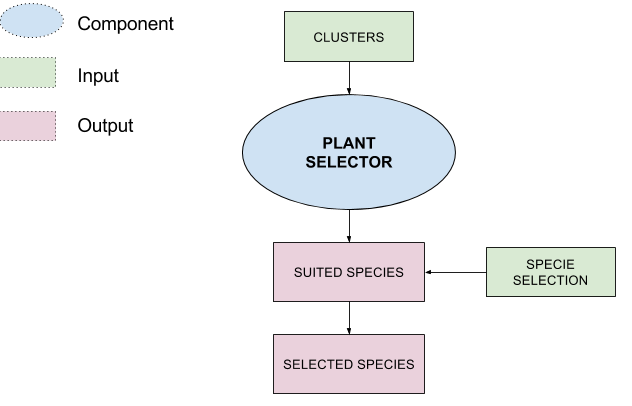
\includegraphics[width=\textwidth]{system_overview_plant_selector.png}
	\caption{ \textit{Plant selector overview.}}	
	\label{fig:system_overview_plant_selector}
\end{figure}

\section{Ecosystem Simulator}

The ecosystem simulator is used to determine a valid plant distribution given a set of plant species and resources (soil humidity, illumination, slope and temperature). It simulates plants spawning, growing, battling and dying through time at monthly intervals on a hundred by hundred metre simulation area. Figure \ref{fig:system_overview_ecosystem_simulator} shows the input and output requirements of this component.

\begin{figure}
\center
	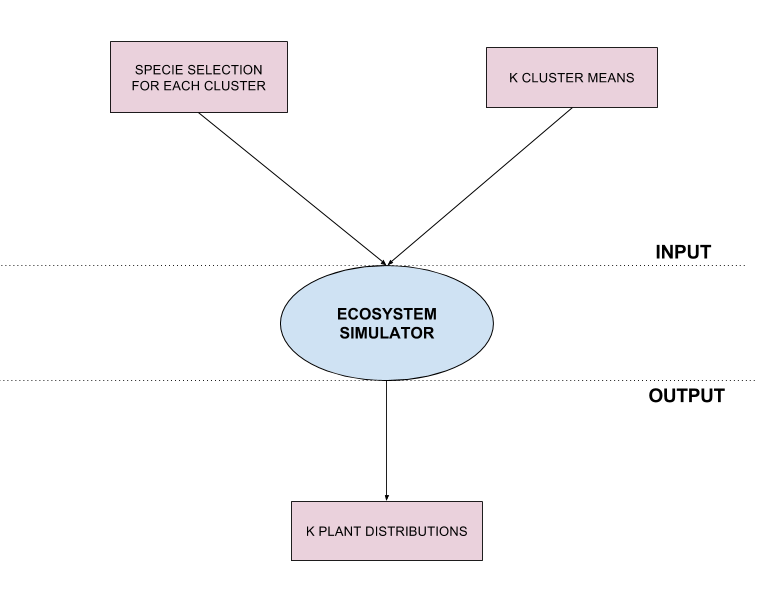
\includegraphics[width=\textwidth]{system_overview_ecosystem_simulator.png}
	\caption{ \textit{Ecosystem simulator overview.}}	
	\label{fig:system_overview_ecosystem_simulator}
\end{figure}

\section{Distribution Analyser and Reproducer}

Because the ecosystem simulator is computationally expensive, the simulation area is restricted to ten thousand square metres (hundred by hundred metres). In order to place vegetation in clusters with larger surface areas, radial distribution analysis and reproduction is performed \cite{Emilien,Boudon2007,Lane2002}. This technique analyses the variation in plant density over distance of an input exemplar in order to generate pair correlation histograms which are used to reproduce distributions matching the characteristics of the input exemplar. Because the reproduction is much less computationally costly than the ecosystem simulator, it is possible to efficiently produce distributions covering much larger areas. Figure \ref{fig:system_overview_distribution_analyser_and_reproducer} shows the input requirements and outputs of this component.

\begin{figure}
\center
	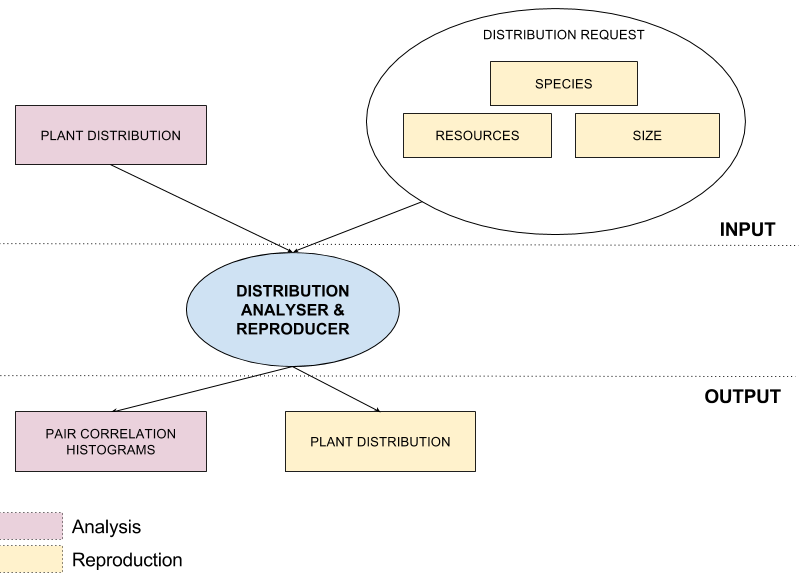
\includegraphics[width=\textwidth]{system_overview_radial_distribution_analyzer_and_reproducer.png}
	\caption{ \textit{Distribution analyser and reproducer overview.}}	
	\label{fig:system_overview_distribution_analyser_and_reproducer}
\end{figure}

\section{Limitations}

The system places vegetation procedurally and does not permit users to place them manually. Unfortunately, this means that fine control over the final vegetation distribution is lost.\\

This work focuses on the generation of untouched rural terrains and does not permit the placement of man-made objects such as roads, cities, buildings and crops. \\

Because of limited scope, the system does not render realistic three dimensional models of the different plants to place on the terrain. The output of the system rather states the position of individual plant instances along with associated properties such as height, root size, canopy width and age.\\

Because of these limitations, it is more accurate to see this system as a tool to be used alongside a game engine such as the \textit{Unreal Engine} \protect\footnotemark \footnotetext{\url{www.unrealengine.com}}. This system could then be used to determine vegetation and water networks on the terrain and the game engine used to generate realistic renders of the scene.

\section{Similarities to Existing Work}

Explicit instancing techniques \cite{Emilien,Deussen1998,Andujar2014} permit users to explicitly state the exact location of individual plant instances. Although this gives users fine-control over terrain content, the task can be long and tedious for very large terrains. Realism can also be poor in these systems as they rely entirely on the user for accurate vegetation placement.\\
Ecosystem simulators techniques ~\cite{Lane2002,Deussen1998} attempt to overcome this by generating plausible plant distributions by algorithmically reproducing the competition for resources that occurs in nature during plant growth. In order to generate plant instances on areas large enough to fill entire terrains in a manageable time frame, however, these algorithms are often over-simplified.\\
Probabilistic placement techniques such as that employed in the work by Emilien et al. \cite{Emilien} attempt to overcome the downside of explicit placement by analysing inter and intra plant distributions in order to replicate similar distributions on much wider areas. This way the user is only required to perform explicit plant placement on a small area, the distribution of which can be analysed and reproduced on any scale with no repetition. Vegetation realism is still not guaranteed, however, as the user is still responsible of producing the input exemplars as well as delimiting areas on the terrain on which to map the exemplar.\\

This work attempts to bridge the gap between ecosystem simulators and probabilistic placement by using the simulator to determine realistic vegetation distributions on a a predefined area and radial distribution analysis to efficiently reproduce it at any scale.\\
By limiting the coverage area of the ecosystem simulator, it is possible to generate more accurate vegetation distributions by performing a more accurate simulation whilst keeping simulation times manageable.\\
A combination of user-focused input tools, procedural methods and an efficient clustering algorithm is used to split the terrain into clusters based on the resources associated with each terrain vertex. By doing so, the system automatically determines the areas of the terrain which differ sufficiently in resources to necessitate a new vegetation distribution to be calculated.\\


